\newpage
\newpage

\begin{minipage}[c]{0.2\textwidth}
\centering
SDGs ONU
\end{minipage}
\fbox{
\begin{minipage}[c]{0.5\textwidth}
\centering
Target ONU 2030
\end{minipage}
}
\begin{minipage}[c]{0.2\textwidth}
\centering
LPT 
\end{minipage}


\begin{minipage}[c]{0.2\textwidth}
    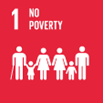
\includegraphics[width=\textwidth]{Images/Social_sustainability/1_no_poverty.png}
\end{minipage}
\fbox{
\begin{minipage}[c]{0.5\textwidth}
1.3 Apply at national level adequate systems and social protection measures for all, including minimum levels, and by 2030 achieve substantial coverage of the poor and vulnerable
\end{minipage}
}
\begin{minipage}[c]{0.2\textwidth}
\emph{Corporate welfare}
\end{minipage}


\begin{minipage}[c]{0.2\textwidth}
    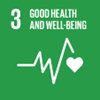
\includegraphics[width=\textwidth]{Images/Social_sustainability/3_helth.png}
\end{minipage}
\fbox{
\begin{minipage}[c]{0.5\textwidth}
3.8 Achieve universal health coverage, including protection from financial risks, access to essential quality health care services and access to safe, effective, quality and affordable essential drugs and vaccines for all
\end{minipage}
}
\begin{minipage}[c]{0.2\textwidth}
\emph{Corporate welfare}
\end{minipage}

\begin{minipage}[c]{0.2\textwidth}
    
\includegraphics[width=\textwidth]{Images/Social_sustainability/white_box.png}
\end{minipage}
\fbox{
\begin{minipage}[c]{0.5\textwidth}
3.6 By 2020, halve the number of deaths and injuries from road traffic accidents worldwide
\end{minipage}
}
\begin{minipage}[c]{0.2\textwidth}
\emph{Health and safety}
\end{minipage}

\begin{minipage}[c]{0.2\textwidth}
    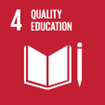
\includegraphics[width=\textwidth]{Images/Social_sustainability/4_education.png}
\end{minipage}
\fbox{
\begin{minipage}[c]{0.5\textwidth}
4.3 By 2030, ensure equal access for all women and men to affordable, high-quality education, vocational and third-level education, including university

4.4 By 2030, substantially increase the number of young people and adults who have the necessary skills, including technical and professional skills, for employment, decent work and entrepreneurial capacity

4.7 By 2030, ensure that all students acquire the knowledge and skills necessary to promote sustainable development through, inter alia, education for sustainable development and sustainable lifestyles, human rights, equality of gender, the promotion of a culture of peace and non-violence, global citizenship and the enhancement of cultural diversity and the contribution of culture to sustainable development
\end{minipage}
}
\begin{minipage}[c]{0.2\textwidth}
\emph{Training and\\ development}
\end{minipage}
\newpage
\begin{minipage}[c]{0.2\textwidth}
\centering
SDGs ONU
\end{minipage}
\fbox{
\begin{minipage}[c]{0.5\textwidth}
\centering
Target ONU 2030
\end{minipage}
}
\begin{minipage}[c]{0.2\textwidth}
\centering
LPT 
\end{minipage}


\begin{minipage}[c]{0.2\textwidth}
    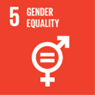
\includegraphics[width=\textwidth]{Images/Social_sustainability/5_gender.png}
\end{minipage}
\fbox{
\begin{minipage}[c]{0.5\textwidth}
5.1 End all forms of discrimination against all women, girls and boys
from all over the world

\end{minipage}
}
\begin{minipage}[c]{0.2\textwidth}
\emph{Training and\\ development}
\end{minipage}

\begin{minipage}[c]{0.2\textwidth}
    
\includegraphics[width=\textwidth]{Images/Social_sustainability/white_box.png}
\end{minipage}
\fbox{
\begin{minipage}[c]{0.5\textwidth}
5.5 Guarantee women full and effective participation and equal leadership opportunities at all levels of decision-making in political, economic and public life
\end{minipage}
}
\begin{minipage}[c]{0.2\textwidth}
\emph{Merit\\ management \\of employee}
\end{minipage}

\begin{minipage}[c]{0.2\textwidth}
    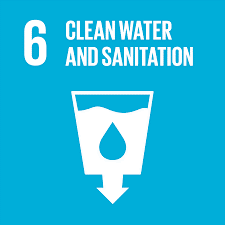
\includegraphics[width=\textwidth]{Images/Social_sustainability/6_water.png}
\end{minipage}
\fbox{
\begin{minipage}[c]{0.5\textwidth}
6.3 By 2030, improve water quality by reducing pollution, eliminating uncontrolled discharge practices and minimizing the release of hazardous chemicals and materials, halve the percentage of untreated wastewater and substantially increase recycling and safe reuse globally

\end{minipage}
}
\begin{minipage}[c]{0.2\textwidth}
\emph{Waste}
\end{minipage}

\begin{minipage}[c]{0.2\textwidth}
    
\includegraphics[width=\textwidth]{Images/Social_sustainability/white_box.png}
\end{minipage}
\fbox{
\begin{minipage}[c]{0.5\textwidth}
6.4 By 2030, substantially increase water efficiency to be used in all sectors and ensure freshwater withdrawals and supplies to address water scarcity and substantially reduce the number of people suffering from water scarcity
\end{minipage}
}
\begin{minipage}[c]{0.2\textwidth}
\emph{Water \\consumption}
\end{minipage}


\begin{minipage}[c]{0.2\textwidth}
    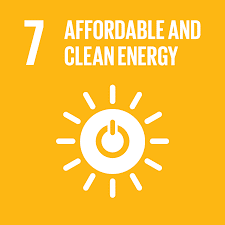
\includegraphics[width=\textwidth]{Images/Social_sustainability/7_energy.png}
\end{minipage}
\fbox{
\begin{minipage}[c]{0.5\textwidth}
7.2 By 2030, significantly increase the share of renewables in the global energy mix

7.3 By 2030, double the global rate of energy efficiency improvement
\end{minipage}
}
\begin{minipage}[c]{0.2\textwidth}
\emph{Energetic\\ consumption}
\end{minipage}

\newpage

\begin{minipage}[c]{0.2\textwidth}
    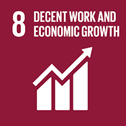
\includegraphics[width=\textwidth]{Images/Social_sustainability/8_work.png}
\end{minipage}
\fbox{
\begin{minipage}[c]{0.5\textwidth}
8.1 Supporting per capita economic growth according to national circumstances and, in particular, at least 7 percent annual growth of gross domestic product in least developed countries
\end{minipage}
}
\begin{minipage}[c]{0.2\textwidth}
\emph{Production and distribution of economic value}
\end{minipage}

\begin{minipage}[c]{0.2\textwidth}
    
\includegraphics[width=\textwidth]{Images/Social_sustainability/white_box.png}
\end{minipage}
\fbox{
\begin{minipage}[c]{0.5\textwidth}
8.2 Achieve higher levels of economic productivity through diversification, technological updating and innovation, including through a focus on high value-added sectors and labour-intensive sectors
\end{minipage}
}
\begin{minipage}[c]{0.2\textwidth}
\emph{Quality of service, customer satisfaction}
\end{minipage}


\begin{minipage}[c]{0.2\textwidth}
    
\includegraphics[width=\textwidth]{Images/Social_sustainability/white_box.png}
\end{minipage}
\fbox{
\begin{minipage}[c]{0.5\textwidth}
8.4 Progressively improve, until 2030, the efficiency of global resources in consumption and production in an attempt to decouple economic growth from environmental degradation, in accordance with the ten-year framework of programs on sustainable consumption and production, with developed countries taking the initiative
\end{minipage}
}
\begin{minipage}[c]{0.2\textwidth}
\emph{Supply-chain management}
\end{minipage}

\begin{minipage}[c]{0.2\textwidth}
    
\includegraphics[width=\textwidth]{Images/Social_sustainability/white_box.png}
\end{minipage}
\fbox{
\begin{minipage}[c]{0.5\textwidth}
8.5 By 2030, achieve full and productive employment and decent work for all women and men, including young people and people with disabilities, and equal pay for work of equal value

8.6 By 2020, substantially reduce the percentage of unemployed young people who do not follow a course of study or who do not follow training courses
\end{minipage}
}
\begin{minipage}[c]{0.2\textwidth}
\emph{Corporate welfare}
\end{minipage}

\begin{minipage}[c]{0.2\textwidth}
    
\includegraphics[width=\textwidth]{Images/Social_sustainability/white_box.png}
\end{minipage}
\fbox{
\begin{minipage}[c]{0.5\textwidth}
8.8 Protect labour rights and promote a safe and secure working environment for all workers, including migrant workers, especially migrant women, and those in precarious work
\end{minipage}
}
\begin{minipage}[c]{0.2\textwidth}
\emph{Health and safety of workers}
\end{minipage}

\newpage

\begin{minipage}[c]{0.2\textwidth}
    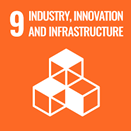
\includegraphics[width=\textwidth]{Images/Social_sustainability/9_industry.png}
\end{minipage}
\fbox{
\begin{minipage}[c]{0.5\textwidth}
9.1 Develop quality, reliable, sustainable and resilient infrastructure, including regional and cross-border infrastructure, to support economic development and human well-being, with a focus on equitable access for all
\end{minipage}
}
\begin{minipage}[c]{0.2\textwidth}
\emph{Quality of service, accessibility, customer satisfaction}
\end{minipage}

\begin{minipage}[c]{0.2\textwidth}
    
\includegraphics[width=\textwidth]{Images/Social_sustainability/white_box.png}
\end{minipage}
\fbox{
\begin{minipage}[c]{0.5\textwidth}
9.5 Strengthen scientific research, promote the technological capacities of industrial sectors in all countries, in particular in developing countries, including by encouraging innovation by 2030 and by substantially increasing the number of workers in the research and development every million people and public and private spending on research and development
\end{minipage}
}
\begin{minipage}[c]{0.2\textwidth}
\emph{Innovation}
\end{minipage}

\begin{minipage}[c]{0.2\textwidth}
    
\includegraphics[width=\textwidth]{Images/Social_sustainability/white_box.png}
\end{minipage}
\fbox{
\begin{minipage}[c]{0.5\textwidth}
9.6 Significantly increase access to information and communication technologies and strive to provide universal and low-cost access to the Internet in least developed countries by 2020
\end{minipage}
}
\begin{minipage}[c]{0.2\textwidth}
\emph{Digital transformation}
\end{minipage}

\begin{minipage}[c]{0.2\textwidth}
    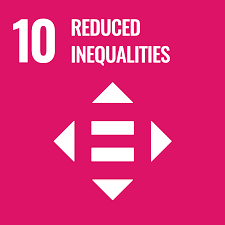
\includegraphics[width=\textwidth]{Images/Social_sustainability/10_ineq.png}
\end{minipage}
\fbox{
\begin{minipage}[c]{0.5\textwidth}
10.3 Ensure equal opportunities for all and reduce result inequalities, including through the elimination of discriminatory laws, policies and practices, and the promotion of adequate laws, policies and actions in this regard

10.4 Adopt policies, in particular fiscal, wage and social protection policies, and progressively achieve greater equality
\end{minipage}
}
\begin{minipage}[c]{0.2\textwidth}
\emph{Evaluation, remuneration and incentive system}
\end{minipage}

\newpage
\begin{minipage}[c]{0.2\textwidth}
    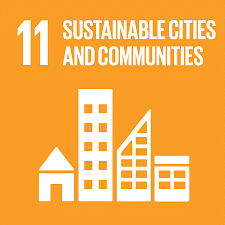
\includegraphics[width=\textwidth]{Images/Social_sustainability/11_cities.png}
\end{minipage}
\fbox{
\begin{minipage}[c]{0.5\textwidth}
11.2 By 2030, provide access to safe, sustainable, and affordable transport systems for all, improve road safety, in particular by expanding public transport, with particular attention to the needs of those in vulnerable situations, women, children, people with disabilities and the elderly
\end{minipage}
}
\begin{minipage}[c]{0.2\textwidth}
\emph{Accessibility of service}
\end{minipage}

\begin{minipage}[c]{0.2\textwidth}
    
\includegraphics[width=\textwidth]{Images/Social_sustainability/white_box.png}
\end{minipage}
\fbox{
\begin{minipage}[c]{0.5\textwidth}
11.3 By 2030, increase inclusive and sustainable urbanization and the capacity for participatory and integrated planning and management of human settlement in all countries
\end{minipage}
}
\begin{minipage}[c]{0.2\textwidth}
\emph{Community}
\end{minipage}

\begin{minipage}[c]{0.2\textwidth}
    
\includegraphics[width=\textwidth]{Images/Social_sustainability/white_box.png}
\end{minipage}
\fbox{
\begin{minipage}[c]{0.5\textwidth}
11.6 By 2030, reduce the negative per capita environmental impact of cities, in particular with regard to air quality and waste management
\end{minipage}
}
\begin{minipage}[c]{0.2\textwidth}
\emph{Emissions}
\end{minipage}

\begin{minipage}[c]{0.2\textwidth}
    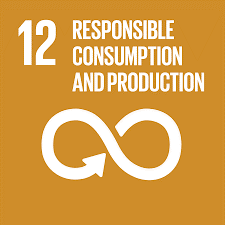
\includegraphics[width=\textwidth]{Images/Social_sustainability/12_consumption.png}
\end{minipage}
\fbox{
\begin{minipage}[c]{0.5\textwidth}
12.2 By 2030, achieve sustainable management and efficient use of natural resources
\end{minipage}
}
\begin{minipage}[c]{0.2\textwidth}
\emph{Consumption of energy and natural resources, waste management}
\end{minipage}

\begin{minipage}[c]{0.2\textwidth}
    
\includegraphics[width=\textwidth]{Images/Social_sustainability/white_box.png}
\end{minipage}
\fbox{
\begin{minipage}[c]{0.5\textwidth}
12.6 Encourage businesses, especially large and transnational companies, to adopt sustainable practices and integrate sustainability information into their reporting
\end{minipage}
}
\begin{minipage}[c]{0.2\textwidth}
\emph{Governance of sustainability and supply chain}
\end{minipage}

\begin{minipage}[c]{0.2\textwidth}
    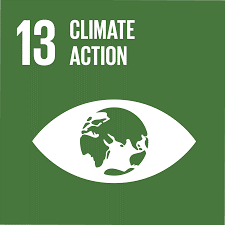
\includegraphics[width=\textwidth]{Images/Social_sustainability/13_climate.png}
\end{minipage}
\fbox{
\begin{minipage}[c]{0.5\textwidth}
13.2 Integrate measures to combat climate change into national policies, strategies and plans
\end{minipage}
}
\begin{minipage}[c]{0.2\textwidth}
\emph{Emission of GHG}
\end{minipage}

\begin{minipage}[c]{0.2\textwidth}
    
\includegraphics[width=\textwidth]{Images/Social_sustainability/16_peace.png}
\end{minipage}
\fbox{
\begin{minipage}[c]{0.5\textwidth}
16.5 Substantially reduce corruption and all its forms

16.4 By 2030, significantly reduce illicit financing and arms trafficking, enhance the recovery and return of stolen assets and fight all forms of organized crime
\end{minipage}
}
\begin{minipage}[c]{0.2\textwidth}
\emph{Community}
\end{minipage}

\begin{minipage}[c]{0.2\textwidth}
    
\includegraphics[width=\textwidth]{Images/Social_sustainability/white_box.png}
\end{minipage}
\fbox{
\begin{minipage}[c]{0.5\textwidth}
16.6 Develop effective, accountable and transparent institutions at all levels
\end{minipage}
}
\begin{minipage}[c]{0.2\textwidth}
\emph{Production and distribution of economic value}
\end{minipage}

\begin{minipage}[c]{0.2\textwidth}
    
\includegraphics[width=\textwidth]{Images/Social_sustainability/white_box.png}
\end{minipage}
\fbox{
\begin{minipage}[c]{0.5\textwidth}
16.7 Ensure responsive, inclusive, participatory and representative decision making at all levels
\end{minipage}
}
\begin{minipage}[c]{0.2\textwidth}
\emph{Customer satisfaction and community attention}
\end{minipage}

\begin{minipage}[c]{0.2\textwidth}
    
\includegraphics[width=\textwidth]{Images/Social_sustainability/white_box.png}
\end{minipage}
\fbox{
\begin{minipage}[c]{0.5\textwidth}
16.8 Promote and enforce non-discriminatory laws and policies for sustainable development
\end{minipage}
}
\begin{minipage}[c]{0.2\textwidth}
\emph{Ethics}
\end{minipage}

\newpage

\begin{minipage}[c]{0.2\textwidth}
    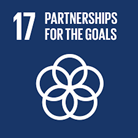
\includegraphics[width=\textwidth]{Images/Social_sustainability/17_partnerships.png}
\end{minipage}
\fbox{
\begin{minipage}[c]{0.5\textwidth}
17.13 Enhance global macro-economic stability, including through policy coordination and coherence

17.14 Improve policy coherence for sustainable development
\end{minipage}
}
\begin{minipage}[c]{0.2\textwidth}
\emph{Community attention}
\end{minipage}

\begin{minipage}[c]{0.2\textwidth}
    
\includegraphics[width=\textwidth]{Images/Social_sustainability/white_box.png}
\end{minipage}
\fbox{
\begin{minipage}[c]{0.5\textwidth}
17.19 By 2030, build, on the basis of existing initiatives, systems for measuring progress towards sustainable development that are complementary to measuring GDP and support the creation of statistical capacity in developing countries

17.17 Encourage and promote effective partnerships in the public sector, between public and private and in civil society based on the experience of partnerships and their ability to find resources
\end{minipage}
}
\begin{minipage}[c]{0.2\textwidth}
\emph{Governance of sustainability}
\end{minipage}


\newpage